\documentclass[onecolumn,preprintnumbers,amsmath,amssymb]{revtex4}
\usepackage{graphicx}
\usepackage{float}
\usepackage[usenames,dvipsnames]{color}

\begin{document}
%\preprint{Draft.13}
\title{Fluctuation of Magnetization}
\author{Cheng Tao Yang$^a$,  Andrew Steinmetz$^a$, Johann Rafelski$^a$}
\affiliation{$^a$Department of Physics, The University of Arizona, Tucson, Arizona 85721, USA}
\date{\today}

%%%%%%%%%%%%%%%%%%%%%%%%%%%%%%%%%%%%%%%%%%%%%%%%%%%%%%%%%%%%%%%%%%

\begin{abstract}
\end{abstract}
\maketitle

\section{Statistical fluctuation of magnetization}
In general, given the magnetic moment $\mu$ the magnetization density of the quantum system is defined as
\begin{align}
\langle M\rangle\equiv\frac{1}{V}\langle \mu\rangle=\frac{1}{V}\left(T\frac{\partial \ln\mathcal Z}{\partial B}\right),\qquad \langle\mu\rangle=\left(T\frac{\partial \ln\mathcal Z}{\partial B}\right)
\end{align}
In statistical mechanical, the mean-square fluctuation of any quantity magnetic moment $\mu$ can be written as
\begin{align}
\langle\Delta \mu^2\rangle=\langle \mu^2\rangle-\langle \mu\rangle^2=T^2\frac{\partial^2 \ln\mathcal Z }{\partial B^2}
\end{align}
In this scenario, the fluctuation of magnetization can be written as
\begin{align}
{\langle\Delta M^2\rangle}=\frac{\langle\Delta \mu^2\rangle}{V}=\frac{T^2}{V}\frac{\partial^2 \ln\mathcal Z }{\partial B^2}=T\frac{\partial}{\partial B}\left(\frac{T}{V}\frac{\partial \ln\mathcal Z}{\partial B}\right)=T\frac{\partial\langle M\rangle}{\partial B}.
\end{align}
%%%%%%%%%%%%%%%%%%%%%%%%%%%%%%%%%%%%%%%%%%%%%%%%%%%%%%%%%%%%%%%%%%%%%%
\section{The fluctuation of magnetized $e^\pm$ plasma }
In our study of magnetization of electron-positron plasma, the partition function of electron-positron plasma is given by
\begin{align}
 \begin{split}
 \label{boltzmann}
 \ln{\cal Z}&\simeq\frac{T^{3}V}{\pi^{2}}\sum_{s'}^{\pm1}\left[\xi_{s'}\cosh{\frac{\mu}{T}}\right]\left(x_{s'}^{2}K_{2}(x_{s'})+\frac{b_{0}}{2}x_{s'}K_{1}(x_{s'})+\frac{b_{0}^{2}}{12}K_{0}(x_{s'})\right)\,,
 \end{split}\\
 \label{xfunc}
 x_{s'}&=\frac{{\tilde m}_{s'}}{T}=\sqrt{\frac{m_{e}^{2}}{T^{2}}+b_{0}\left(1-\frac{g}{2}s'\right)},\,\qquad b_0=\frac{eB}{T^2}.
\end{align}
We show that the total dimensionless magnetization ${\mathfrak M}$  for the case $g=2$ can be broken into the sum of magnetic moment parallel ${\mathfrak M}_{+}$ and magnetic moment anti-parallel ${\mathfrak M}_{-}$ contributions as follows
\begin{align}
\label{g2mag}
{\mathfrak M}={\mathfrak M}_{+}+{\mathfrak M}_{-},\,\qquad {\mathfrak M}=\frac{e\langle M\rangle}{m_e^2},\qquad \langle M\rangle=\frac{T}{V}\frac{\partial \ln{\mathcal Z}}{\partial B},\end{align}
where ${\mathfrak M}_{+}$ and ${\mathfrak M}_{-}$ are given by
\begin{align}
{\mathfrak M}_{+}&=\frac{e^{2}}{\pi^{2}}\frac{T^{2}}{m_{e}^{2}}\xi\cosh{\frac{\mu}{T}}\left[\frac{1}{2}x_{+}K_{1}(x_{+})+\frac{b_{0}}{6}K_{0}(x_{+})\right],\qquad x_{+}=\frac{m_{e}}{T},
\end{align}
and 
\begin{align}
{\mathfrak M}_{-}&=-\frac{e^{2}}{\pi^{2}}\frac{T^{2}}{m_{e}^{2}}\xi^{-1}\cosh{\frac{\mu}{T}}\left[\left(\frac{1}{2}+\frac{b_{0}^{2}}{12x_{-}^{2}}\right)x_{-}K_{1}(x_{-})+\frac{b_{0}}{3}K_{0}(x_{-})\right],  \qquad x_{-}=\sqrt{\frac{m_{e}^{2}}{T^{2}}+2b_{0}}
 \end{align}
 In this scenario, the fluctuation of magnetized electron-positron plasma can be obtain 
 \begin{align}
 \langle\Delta {M}^2\rangle=T\frac{\partial {\langle M\rangle} }{\partial B}=T\frac{\partial b_0}{\partial B}\frac{\partial {\langle M\rangle} }{\partial b_0}=T\left(\frac{e}{T^2}\right)\frac{\partial}{\partial b_0}\left(\frac{m^2_e}{e}{\mathfrak M}\right)=\frac{m_e^2}{T}\left(\frac{\partial {\mathfrak M}_{+} }{\partial b_0}+\frac{\partial {\mathfrak M} _{-}}{\partial b_0}\right)
 \end{align}
 where 
 \begin{align}
 \frac{\partial {\mathfrak M}_{+} }{\partial b_0}=\frac{e^{2}}{\pi^{2}}\frac{T^{2}}{m_{e}^{2}}\xi\cosh{\frac{\mu}{T}}\,\left[\frac{1}{6}K_{0}(x_{+})\right],\qquad x_{+}=\frac{m_{e}}{T}
 \end{align}
 and 
 \begin{align}
  \frac{\partial {\mathfrak M}_{-} }{\partial b_0}=\frac{e^{2}}{\pi^{2}}\frac{T^{2}}{m_{e}^{2}}\xi^{-1}\cosh{\frac{\mu}{T}}\left[\left(\frac{1}{6}+\frac{b^2_0}{12x^2_{-}}\right)K_0(x_{-})+\left(\frac{b_0}{6x_{-}}+\frac{b^2_0}{6x^3_{-}}\right)K_1(x_{-})\right],\qquad  x_{-}=\sqrt{\frac{m_{e}^{2}}{T^{2}}+2b_{0}}
 \end{align}
In Fig.~\ref{Susc_fig} we plot the $\partial{\mathfrak M}_\pm/\partial b_0$ of the primordial $e^{+}e^{-}$-plasma as a function of temperature, with $g=2$, $\xi=1$, $b_0=10^{-11}$ and $b_0=10^{-3}$. It shows that in the magnetic field we consider $10^{-11}<b_0<10^{-3}$, the dominate term for $\partial{\mathfrak M}_{-}/\partial b_0$ is given by
 \begin{align}
\frac{\partial {\mathfrak M}_{-} }{\partial b_0}&\approx\frac{e^{2}}{\pi^{2}}\frac{T^{2}}{m_{e}^{2}}\xi^{-1}\cosh{\frac{\mu}{T}}\left[\left(\frac{1}{6}\right)K_0(x_{-})\right]\approx \frac{\partial {\mathfrak M}_{+} }{\partial b_0}, \qquad \mathrm{for} \,\,10^{-11}<b_0<10^{-3},
 \end{align}
 then the fluctuation of magnetized electron-positron plasma can be approximated by
 \begin{align}
  \langle\Delta {M}^2\rangle=\frac{m_e^2}{T}\left(\frac{\partial {\mathfrak M}_{+} }{\partial b_0}+\frac{\partial {\mathfrak M} _{-}}{\partial b_0}\right)\approx \frac{T}{6}\left(\frac{e^{2}}{\pi^{2}}\right)\cosh{\frac{\mu}{T}}\bigg[\xi K_0(x_+)+\xi^{-1}K_0(x_{-})\bigg]
 \end{align} 
 In Fig.~\ref{Flu_fig} we plot the fluctuation $ \langle\Delta {\mathcal M}^2\rangle/m_e$ nd  $\langle\Delta {\mathcal M}^2\rangle/\sqrt{\langle M\rangle}$ as a function of temperature with $g=2$,  $\xi=1$, $b_0=10^{-11}$ and $b_0=10^{-3}$.

 
 %~~~Figure~~~~~~~~~~~~~~~~~~~~~~~~~~~~~~~~~~~~~~~~~~~~~~~~~
 \begin{figure}[ht]
 \centering
 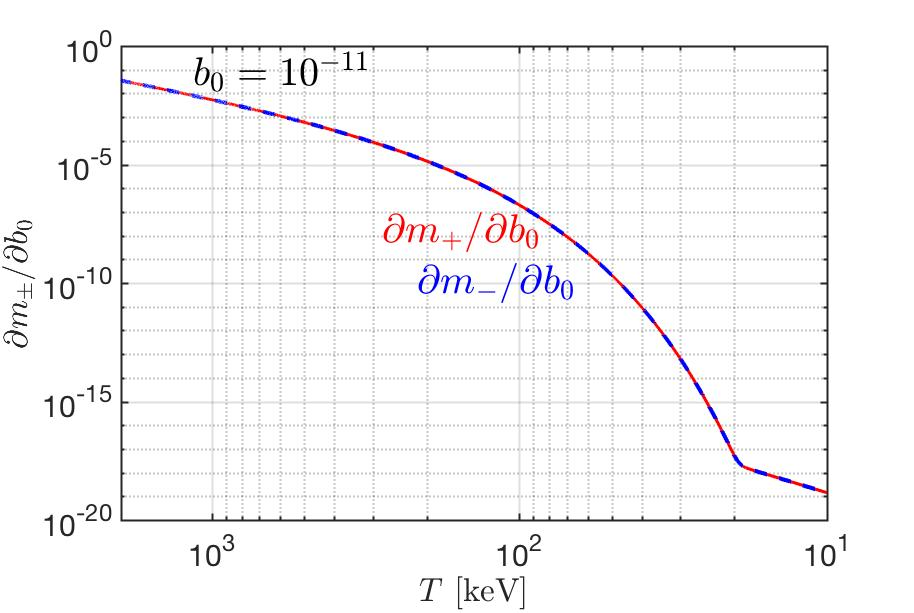
\includegraphics[width=0.5\textwidth]{Susceptibility001}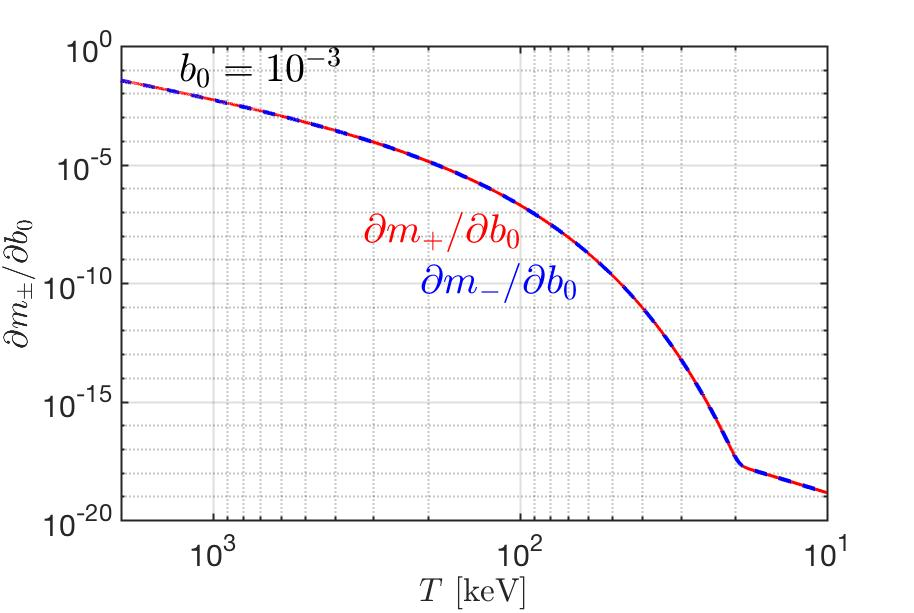
\includegraphics[width=0.5\textwidth]{Susceptibility002}
 \caption{The  $\partial{\mathfrak M}_\pm/\partial b_0$ of the primordial $e^{+}e^{-}$-plasma as a function of temperature, with $g=2$,  $\xi=1$, $b_0=10^{-11}$ and $b_0=10^{-3}$.} 
\label{Susc_fig} 
\end{figure}
 %~~~Figure~~~~~~~~~~~~~~~~~~~~~~~~~~~~~~~~~~~~~~~~~~~~~~~~~

  %~~~Figure~~~~~~~~~~~~~~~~~~~~~~~~~~~~~~~~~~~~~~~~~~~~~~~~~
 \begin{figure}[ht]
 \centering
 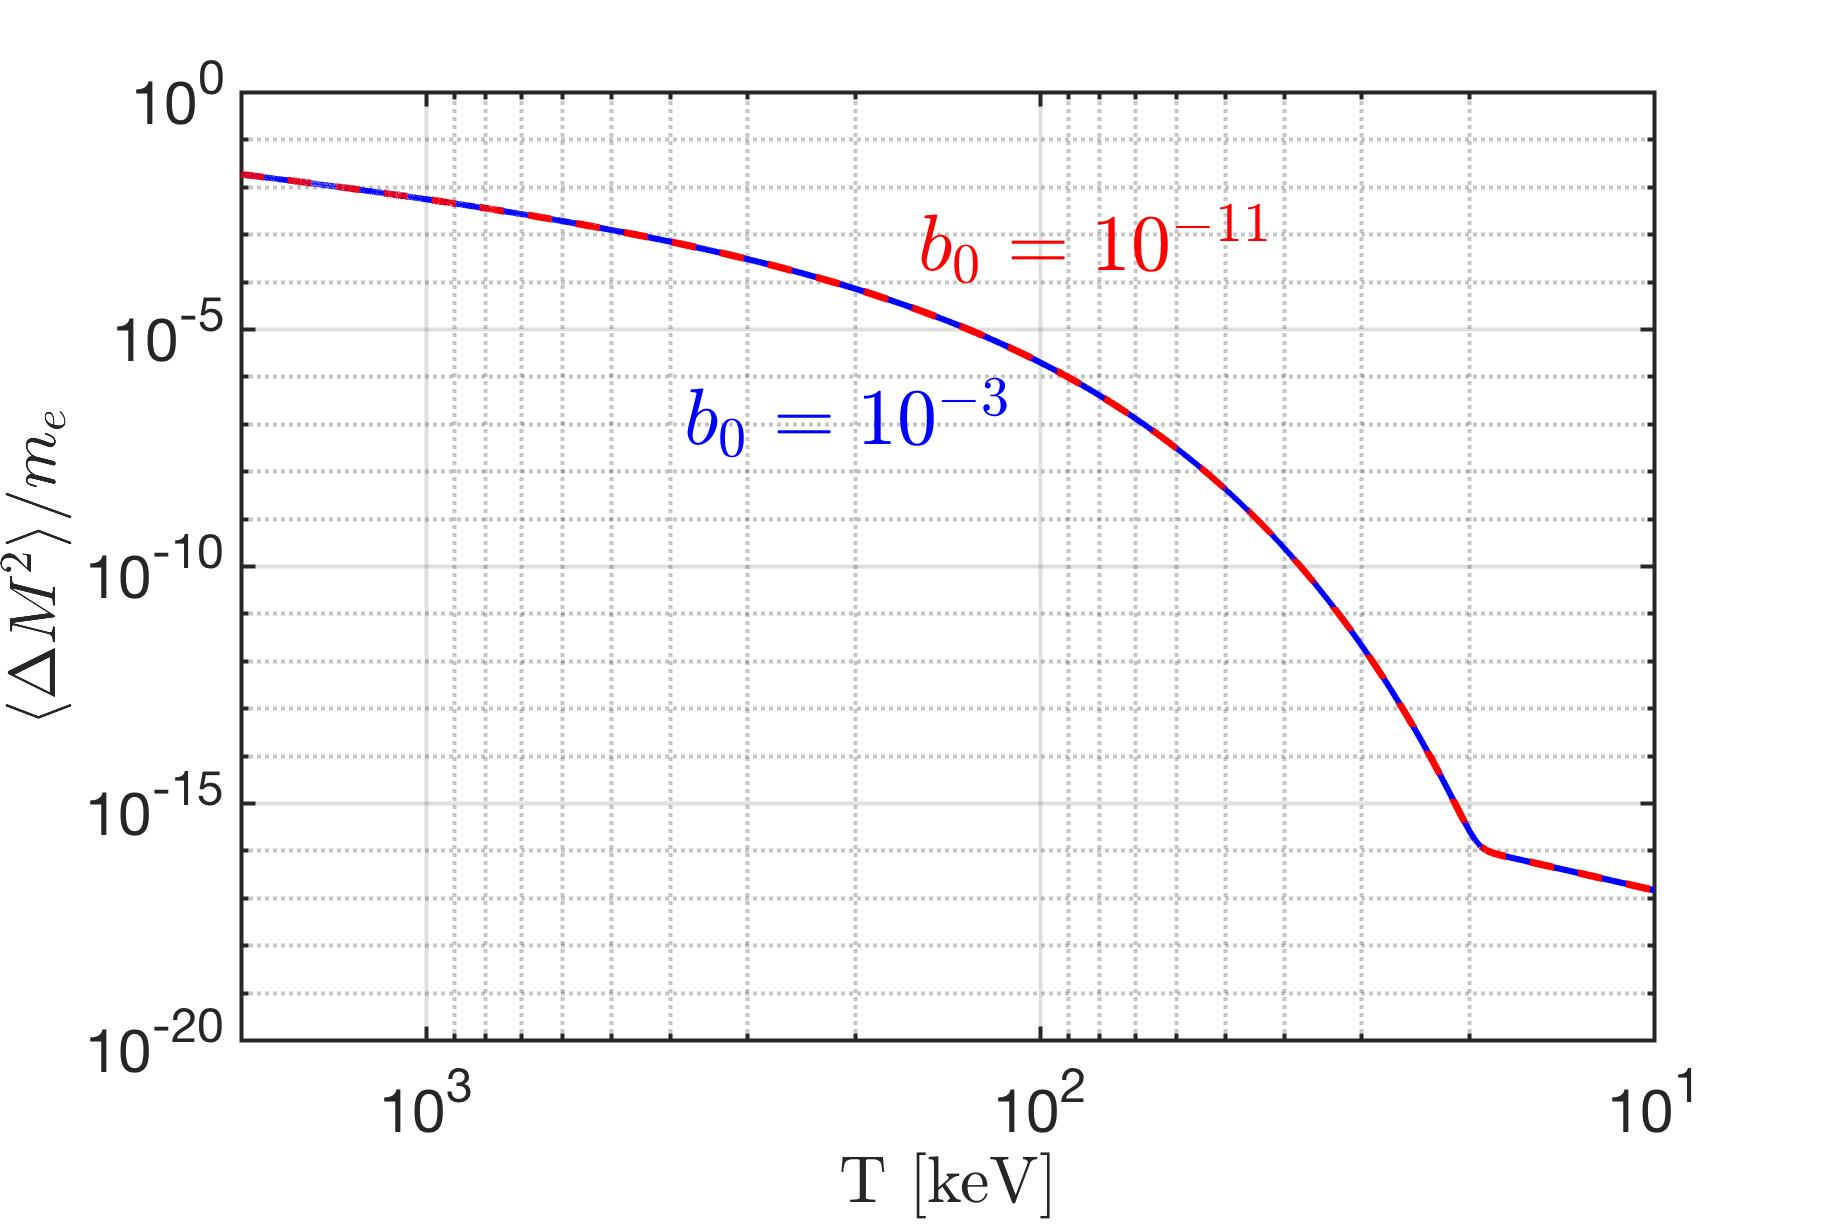
\includegraphics[width=0.5\textwidth]{Fluctuation_Magnetization}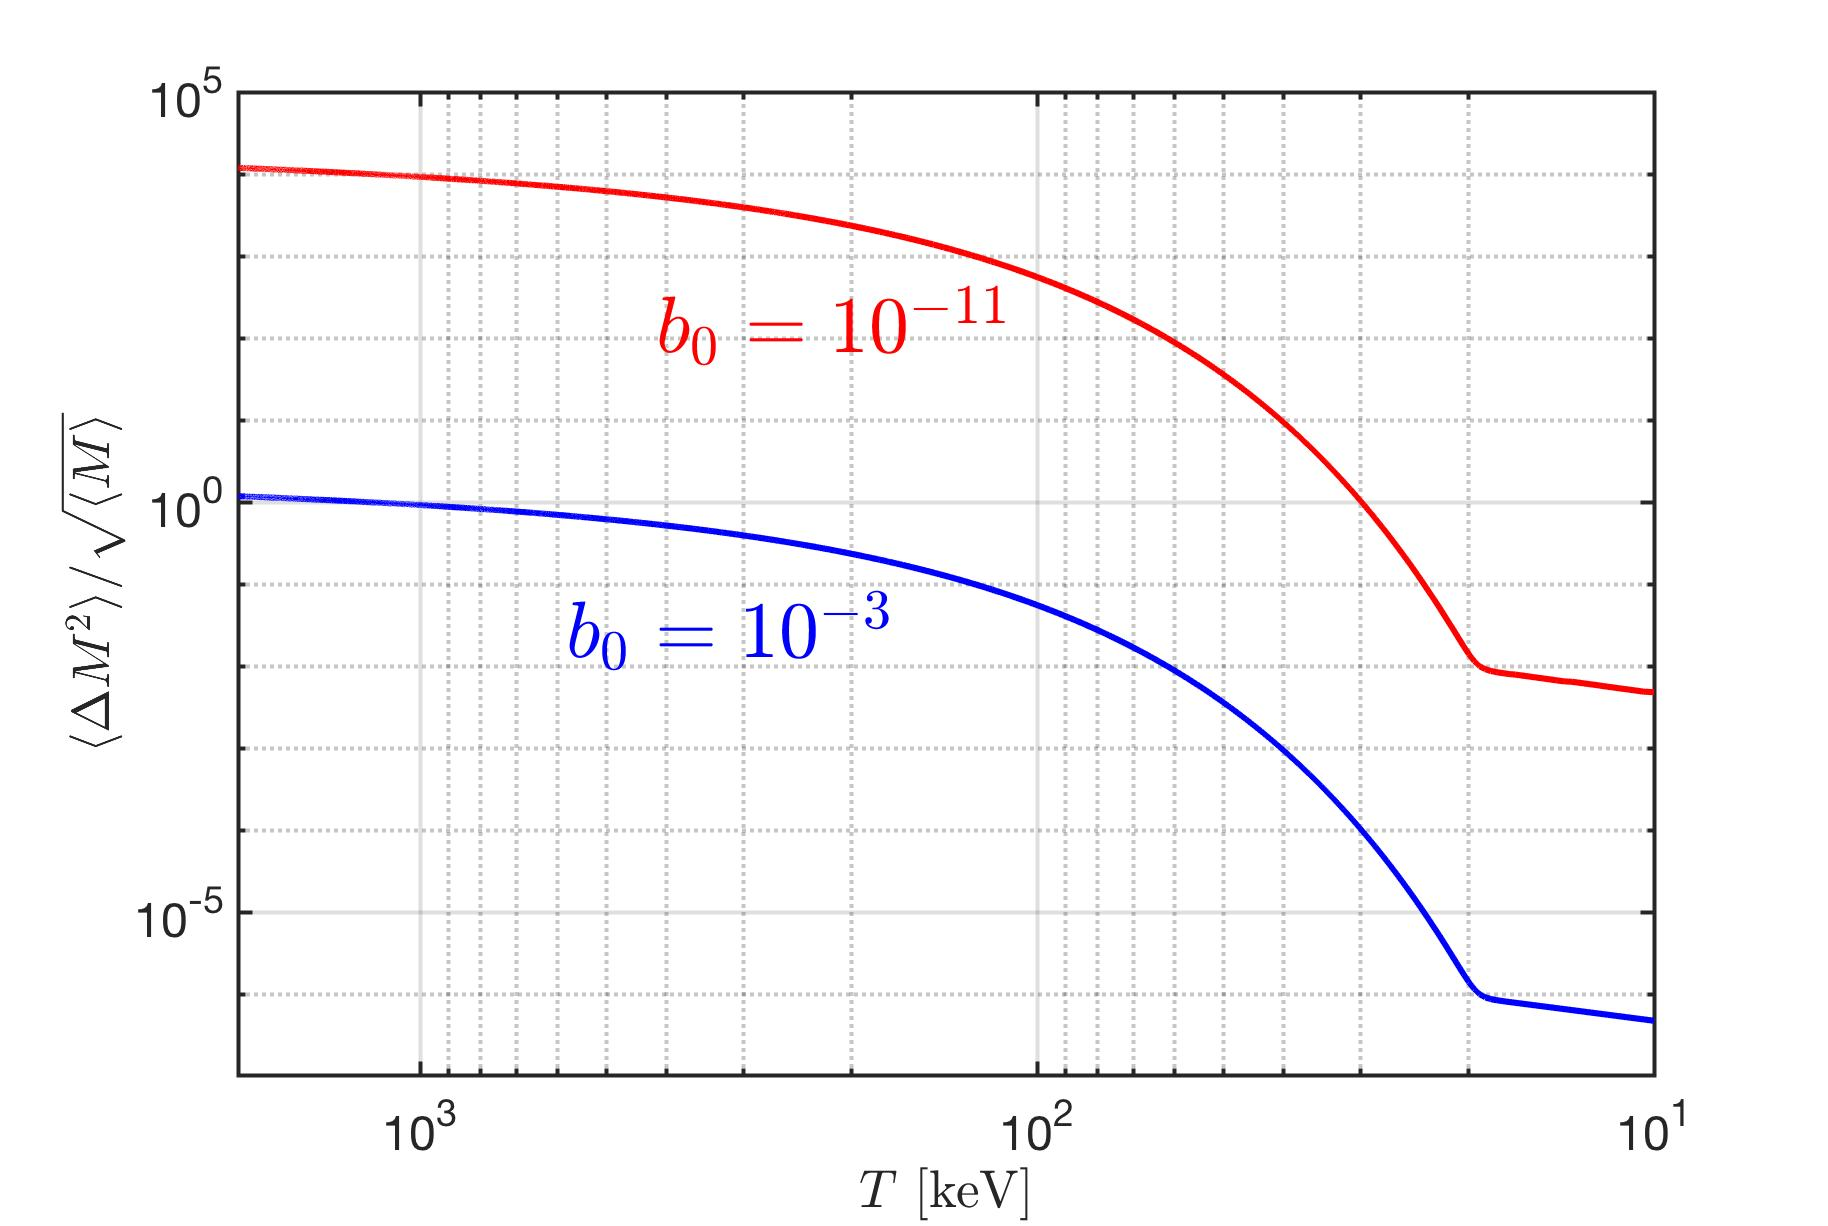
\includegraphics[width=0.5\textwidth]{Fluctuation_M002}
 \caption{The  dimensionless fluctuation $ \langle\Delta {M}^2\rangle/m_e$  and  $\langle\Delta {\mathcal M}^2\rangle/\sqrt{\langle M\rangle}$ of the primordial $e^{+}e^{-}$-plasma as a function of temperature, with $g=2$,  $\xi=1$, $b_0=10^{-11}$ and $b_0=10^{-3}$.} 
 \label{Flu_fig} 
\end{figure}
 
 %~~~Figure~~~~~~~~~~~~~~~~~~~~~~~~~~~~~~~~~~~~~~~~~~~~~~~~~

 %%%%%%%%%%%%%%%%%%%%%%%%%%%%%%%%%%%%%%%%%%%%%%%%%%%%%%%%%%%%%%%%%%%%%%

\begin{thebibliography}{99}
 \end{thebibliography}
%%%%%%%%%%%%%%%%%%%%%%%%%%%%%%%%%%%%%%%%%%%%%%%%%%%%%%%%%%%%%%%%%%%
\end{document} 